% !TeX encoding = utf8


\documentclass{standalone}
\usepackage{circuitikz}
\begin{document}
    % Insert figure here
    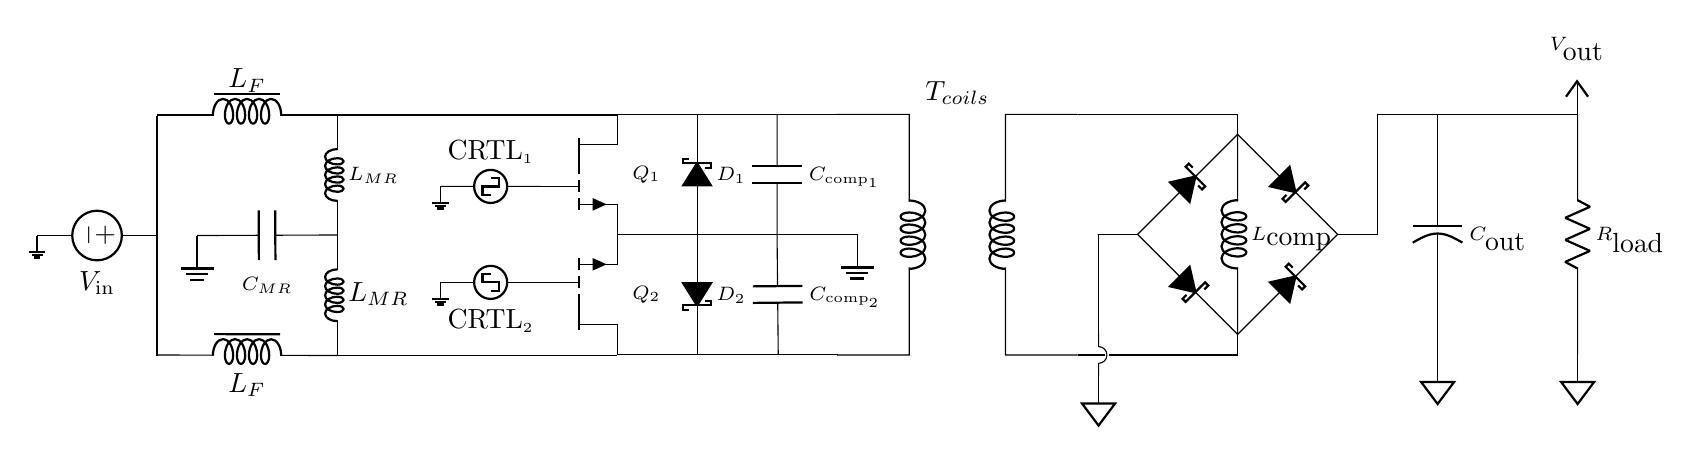
\begin{tikzpicture}
        % Paths, nodes and wires:
        \node[GaN hemt, xscale=0.99, yscale=0.99](N1) at (7.366, 2.301){} node[anchor=west] at (N1.text){$\scriptstyle{Q_1}$};
        \node[transformer, cute, xscale=1.455, yscale=1.455](N2) at (11.688, 1.535){} node[anchor=south] at (N2.text){$T_{coils}$};
        \draw (8.382, 1.539) to[full Schottky diode, /tikz/circuitikz/bipoles/length=0.700cm, l_={$\scriptstyle{D_1}$}] (8.382, 3.063);
        \draw (13.977, 1.539) to[full Schottky diode, /tikz/circuitikz/bipoles/length=0.700cm] (15.247, 2.809);
        \draw (15.247, 2.809) to[full Schottky diode, /tikz/circuitikz/bipoles/length=0.700cm] (16.517, 1.539);
        \draw (13.977, 1.539) to[full Schottky diode, /tikz/circuitikz/bipoles/length=0.700cm] (15.247, 0.269);
        \draw (15.247, 0.269) to[full Schottky diode, /tikz/circuitikz/bipoles/length=0.700cm] (16.517, 1.539);
        \draw (15.247, 0.269) to[cute inductor, l_={$\scriptstyle{L_\textrm{comp}}$}] (15.247, 2.809);
        \node[GaN hemt, xscale=0.99, yscale=-0.99](N3) at (7.366, 0.777){} node[anchor=west] at (N3.text){$\scriptstyle{Q_2}$};
        \draw (8.382, 1.539) to[full Schottky diode, mirror, /tikz/circuitikz/bipoles/length=0.700cm, l={$\scriptstyle{D_2}$}] (8.382, 0.015);
        \node[ground] at (10.414, 1.539){};
        \node[jump crossing, rotate=-90, xscale=1.9, yscale=1.9] at (13.481, 0.007){};
        \node[sground] at (13.481, -0.259){};
        \draw (13.747, 0.007) -| (15.247, 0.015) -| (15.247, 0.269);
        \draw (13.481, 0.273) |- (13.469, 1.539) -- (13.977, 1.539);
        \draw (13.215, 3.063) -- (15.247, 3.063) -| (15.247, 2.809);
        \node[vcc](N4) at (19.558, 3.063){} node[anchor=south] at (N4.text){$\scriptstyle{V_\textrm{out}}$};
        \draw (16.517, 1.539) -- (17.025, 1.539) -| (17.025, 2.809) -| (17.025, 3.063) -- (17.787, 3.063);
        \node[sground] at (17.787, 0.015){};
        \draw (19.565, 3.063) to[american resistor, /tikz/circuitikz/bipoles/length=1.05cm, l={$\scriptstyle{R_\textrm{load}}$}] (19.565, 0.015);
        \node[sground] at (19.565, 0.015){};
        \draw (17.787, 3.063) -- (19.565, 3.063);
        \draw (5.126, 2.148) to[square voltage source, /tikz/circuitikz/bipoles/length=0.700cm, l={$\scriptscriptstyle{\textrm{CRTL}_1}$}] (6.396, 2.148);
        \draw (5.126, 0.929) to[square voltage source, mirror, /tikz/circuitikz/bipoles/length=0.700cm, l_={$\scriptscriptstyle{\textrm{CRTL}_2}$}] (6.396, 0.929);
        \node[ground, xscale=0.5, yscale=0.5] at (5.126, 0.929){};
        \node[ground, xscale=0.5, yscale=0.5] at (5.126, 2.148){};
        \draw (9.398, 3.063) to[capacitor, /tikz/circuitikz/bipoles/length=1.05cm, l={$\scriptstyle{C_\mathrm{comp_1}}$}] (9.398, 1.539);
        \draw (9.398, 1.539) to[capacitor, /tikz/circuitikz/bipoles/length=1.05cm, l={$\scriptstyle{C_\mathrm{comp_2}}$}] (9.413, 0.014);
        \draw (17.787, 3.063) to[curved capacitor, /tikz/circuitikz/bipoles/length=1.05cm, l={$\scriptstyle{C_\textrm{out}}$}] (17.787, 0.015);
        \draw (7.366, 0.014) -| (8.382, 0.015) -| (9.413, 0.014) -| (10.16, 0.007);
        \draw (7.366, 1.538) -| (8.382, 1.539) -- (9.398, 1.539) -- (10.414, 1.539);
        \draw (7.366, 3.063) -- (8.382, 3.063) -- (9.398, 3.063) -- (10.16, 3.063);
        \draw (1.524, 3.055) to[cute choke, l={$L_F$}] (3.81, 3.055);
        \draw (1.524, 0.007) to[cute choke, l_={$L_F$}] (3.81, -0);
        \draw (3.81, 1.531) to[cute inductor, /tikz/circuitikz/bipoles/length=1.05cm, l_={$\scriptstyle{L_{MR}}$}] (3.81, 3.055);
        \draw (3.81, -0) to[cute inductor, /tikz/circuitikz/bipoles/length=1.05cm, l_={$L_{MR}$}] (3.81, 1.531);
        \draw (1.524, 1.524) to[american voltage source, /tikz/circuitikz/bipoles/length=1.05cm, l={$V_\mathrm{in}$}] (0, 1.524);
        \node[ground, xscale=0.5, yscale=0.5] at (0, 1.524){};
        \draw (3.81, 1.531) to[capacitor, /tikz/circuitikz/bipoles/length=1.05cm, l={$\scriptstyle{C_{MR}}$}] (2.032, 1.524);
        \node[ground] at (2.032, 1.524){};
        \draw (1.524, 3.048) -| (1.524, 1.524) -- (1.524, -0);
        \draw (3.81, 3.055) -| (7.366, 3.063);
        \draw (7.366, -0) -- (3.81, -0);
    \end{tikzpicture}
\end{document}